\clearpage
\section{Physical channel6: ADC PASS; integrator qualification incomplete}
Both USB pairs moved7 to6, DAC0/1 to J8 and2/3 to J6. Active/inhibited probes
verified routing; MCU1803, FPGA ff2f746c and power guards passed. No programming,
clock-profile changes, Kasli output release or SMU access.
\subsection{ADC transfer and adjacent bits: PASS}
Both257-point sweeps use differential range plus/minus1.2V, common mode1V,
outputs0.4--1.6V. All bits and44adjacent-pair states exercised. Frozen channel8
source/method contracts matched. Previous selected results unchanged.
\begin{center}\begin{tabular}{lrrr}\toprule
ADC & Gain(code/V) & Zero mean(code) & Template-removed RMS(code)\\\midrule
A & -1776.21 & 2177.935 & 0.633 \\
B & -1768.63 & 2168.362 & 0.553 \\
\bottomrule\end{tabular}\end{center}
\begin{center}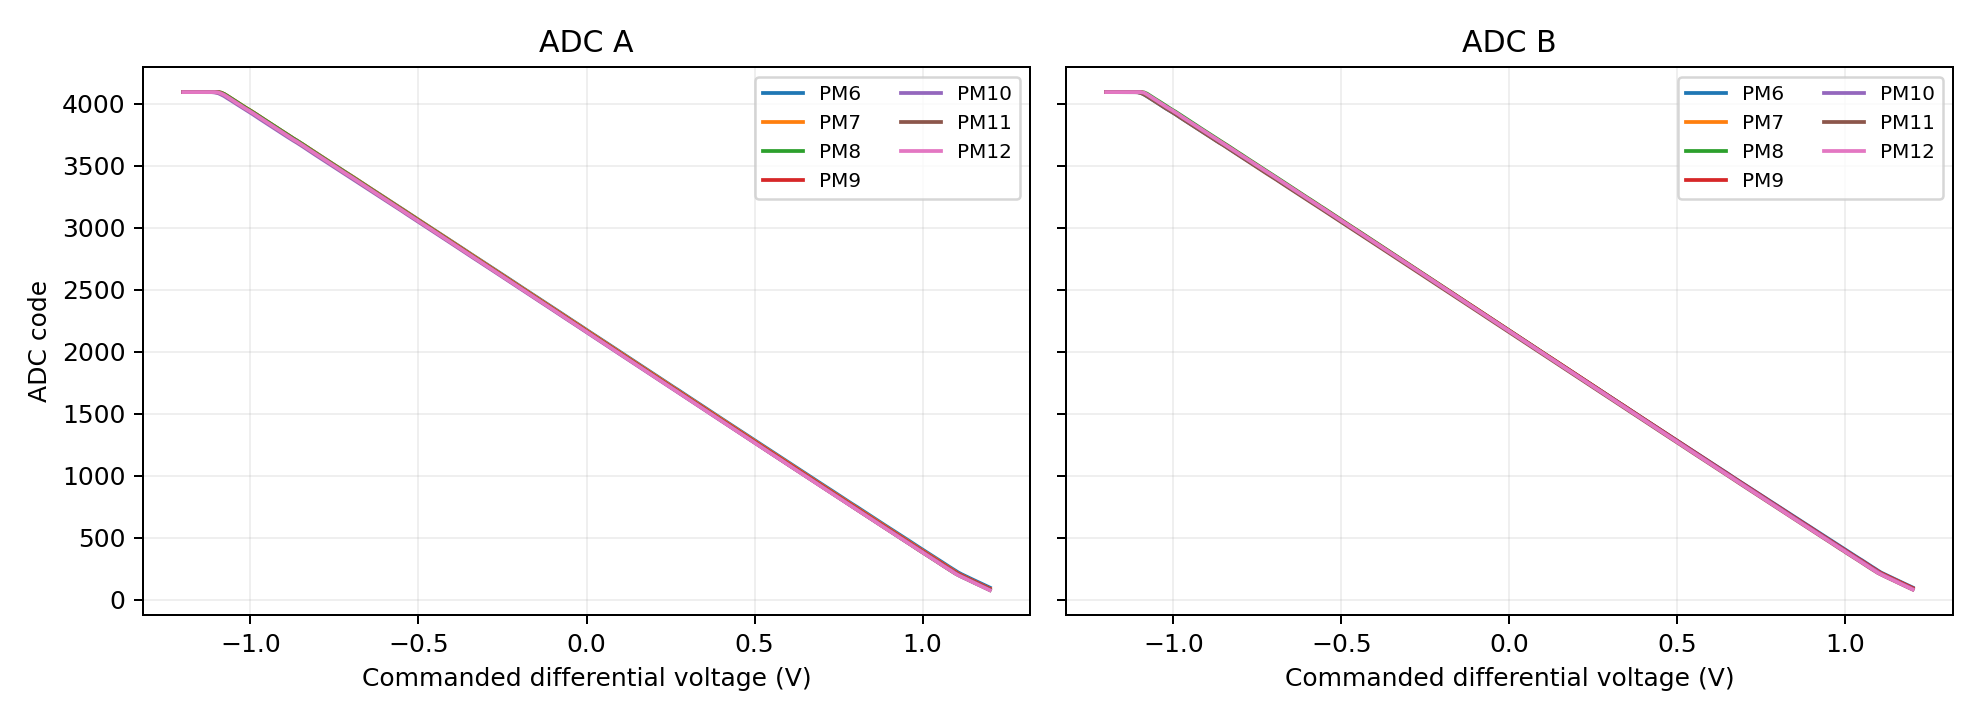
\includegraphics[width=\linewidth]{ch06-adc-dc-06-12.png}\end{center}
Whole-chain commanded-voltage response, not calibrated ADC-only gain.
Older10--12 use c7c42d28;6--9 use ff2f746c; individual receipts retain conditions.
\subsection{Integrator: INCOMPLETE, not a hardware failure determination}
The13-point coarse sweep completed. A shows a signed reversal, but B lacks a
separated integration/reset template near balance. The controller stopped before
fine/return qualification. Four additional DAC-A phase settings did not remove
this ambiguity; raw data retained, thresholds unchanged, DAC-A restored0.
Both-bank qualification remains incomplete; no balance or gain for B is reported.
\begin{center}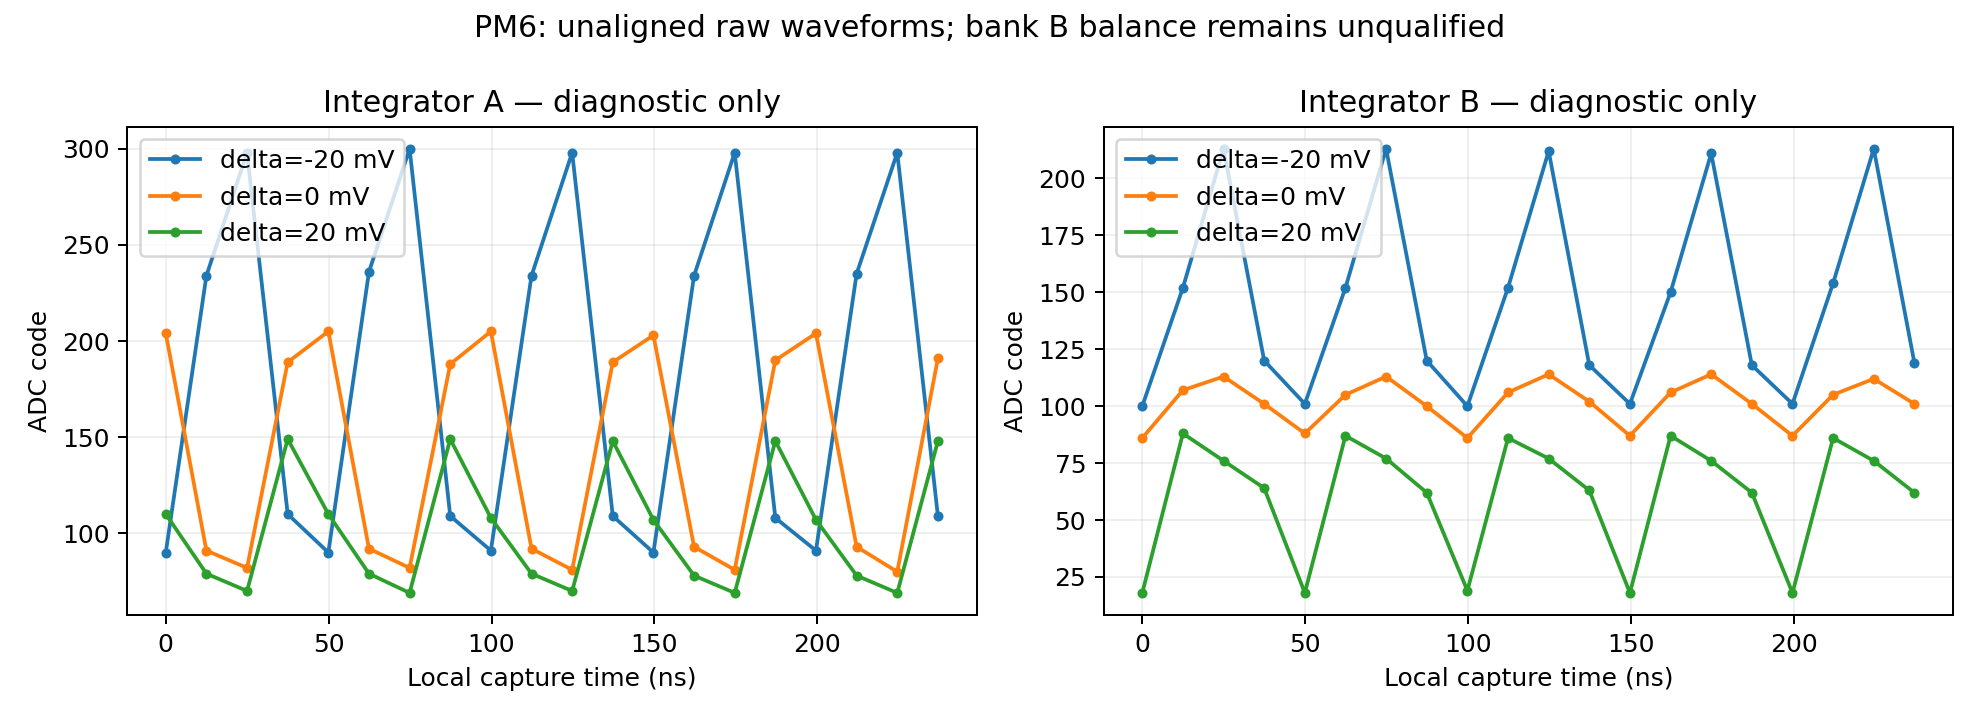
\includegraphics[width=\linewidth]{ch06-integrator-diagnostic.png}\end{center}
Raw waveforms have separate local capture origins, not a shared trigger.
Final channel6 amplifiers disabled, direct bypass inhibited, all monitor muxes
inhibited; TCA masks are zero. External DAC channels 0/1 are 1/1 V;
channels 2/3 are 1.024/2.048 V. Kasli outputs are unchanged;
leases released. Channel5 analog tests still await the USB move.

\subsection{Zero-input waveforms and FFT}
Selected zero-differential buffers for channels6--12 are compared below.
Capture origins are local, not synchronized. FFT amplitudes are one-sided RMS
code per bin at nominal80.1574MS/s, not spectral density or intrinsic aperture jitter.
\begin{center}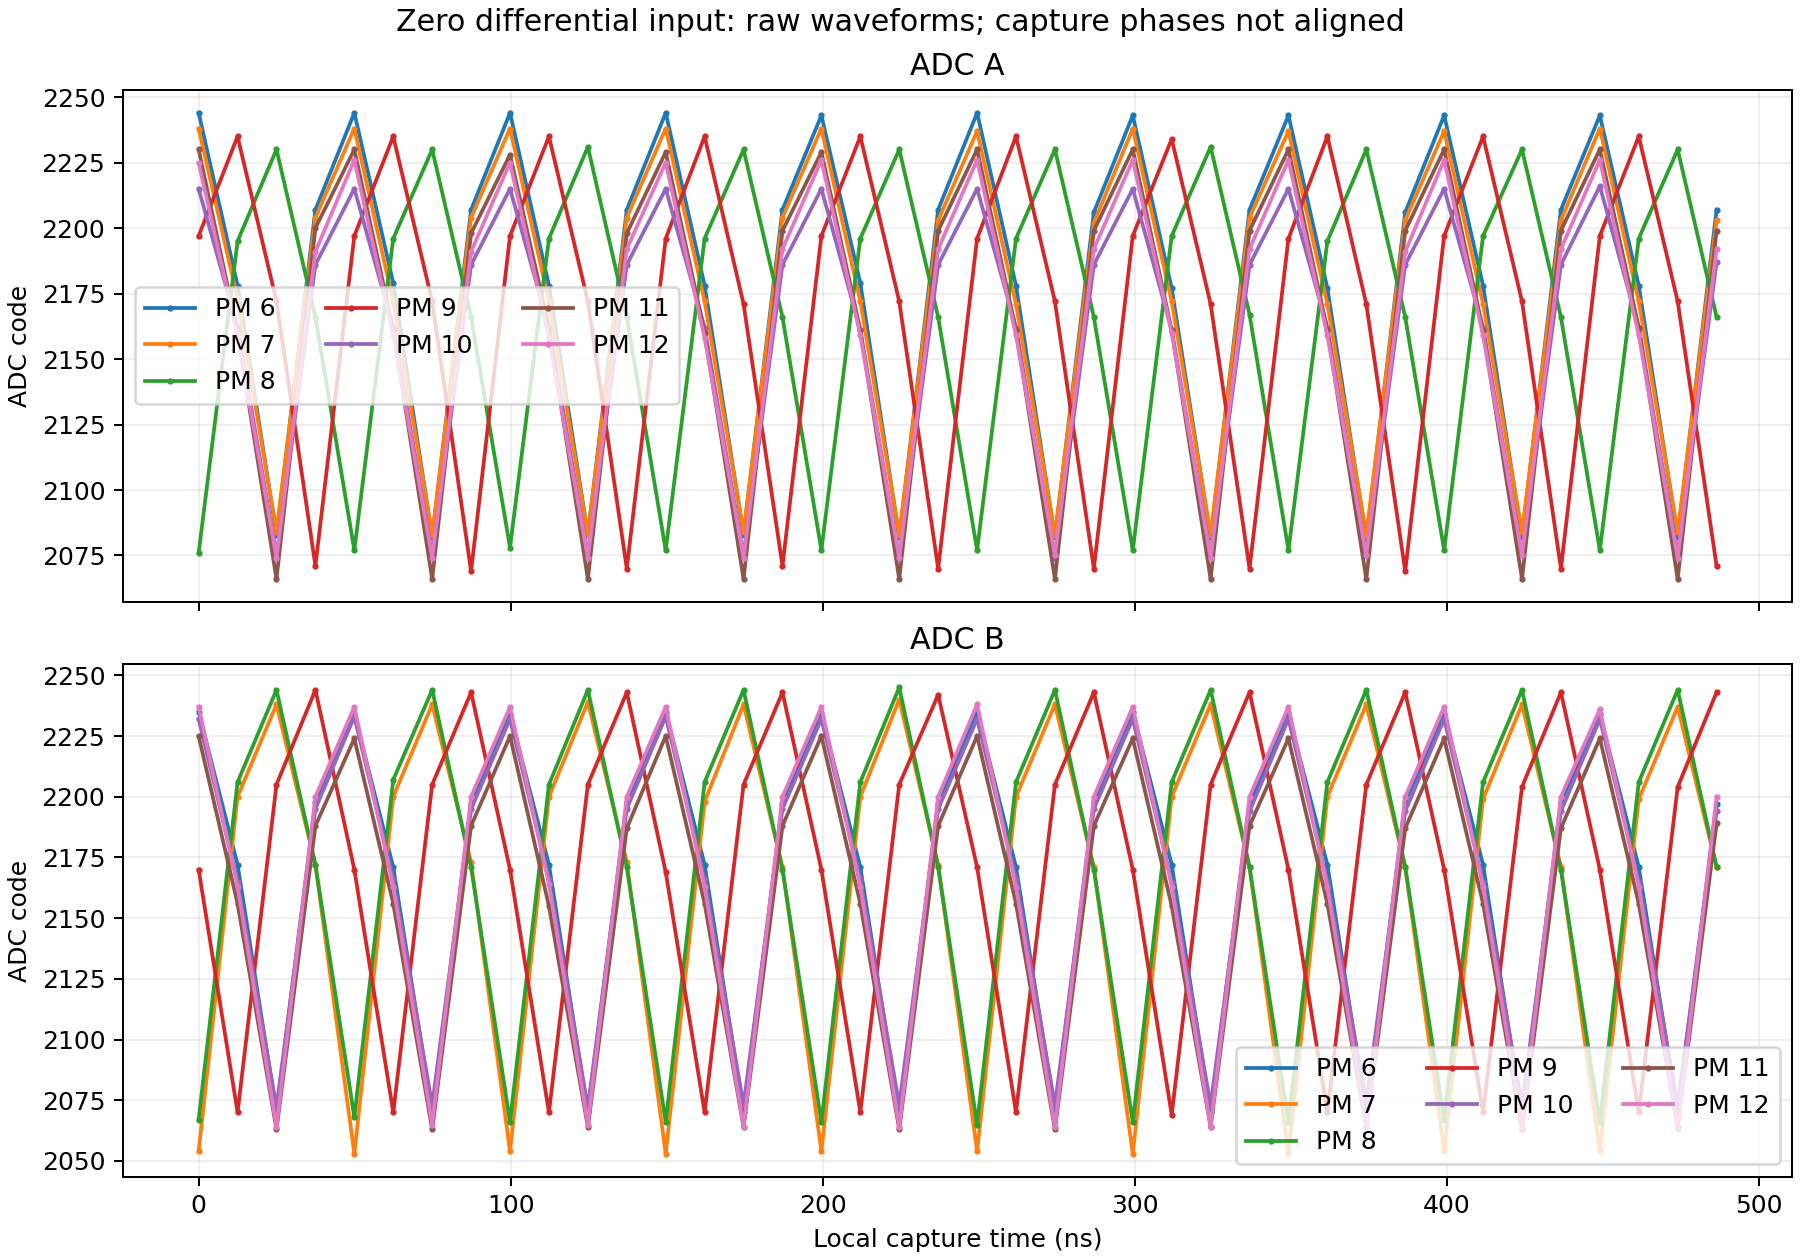
\includegraphics[width=\linewidth]{ch06-adc-zero-time.png}\end{center}
\begin{center}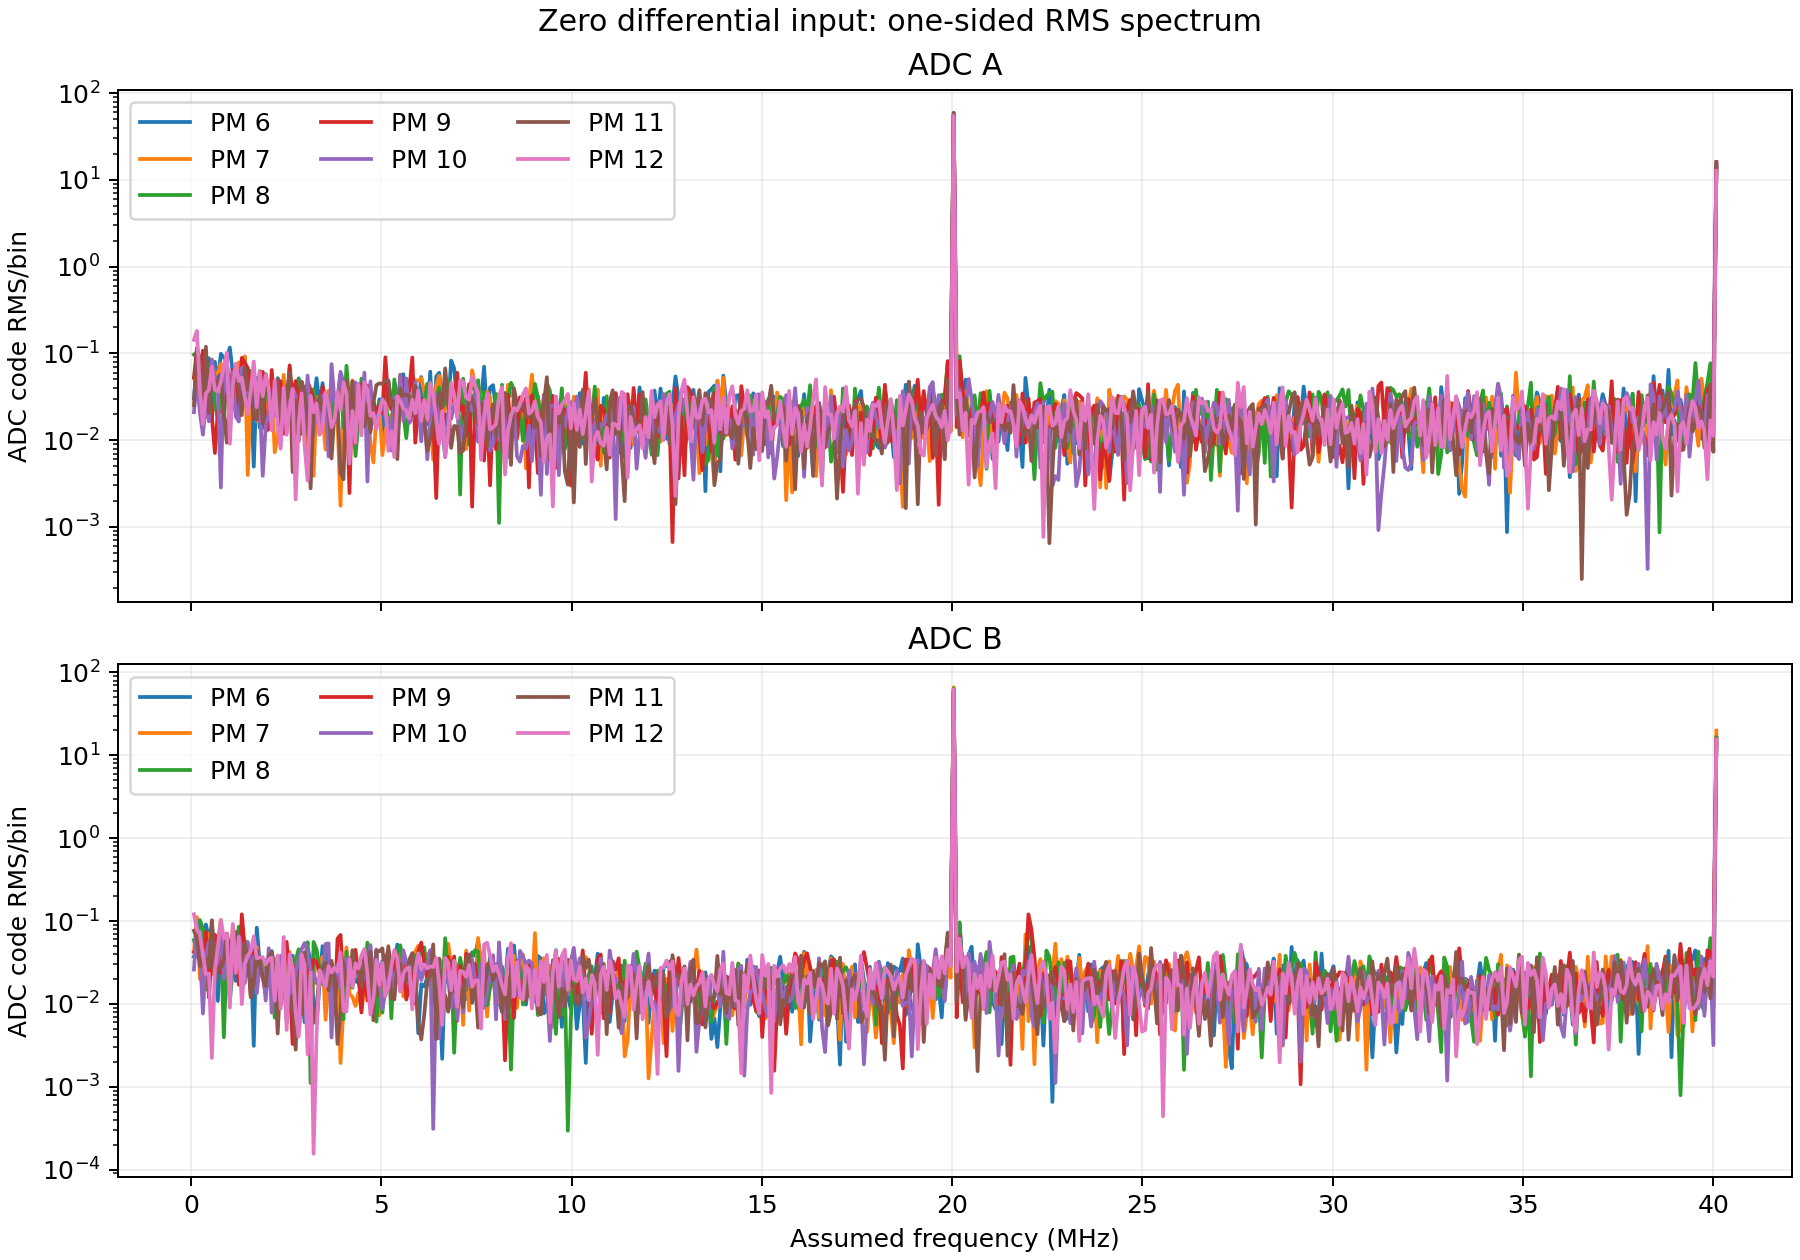
\includegraphics[width=\linewidth]{ch06-adc-zero-fft.png}\end{center}
